% 41039 Programming 1 revision; shared style copied from the established Week 4 deck.
\documentclass[aspectratio=169]{beamer}
\makeatletter

\usepackage{lmodern}
\usepackage{booktabs}
\usepackage{array}
\usepackage{graphicx}
\usepackage{xcolor}
\usepackage{listings}
\usepackage{pifont}
\usepackage{enumitem}
\usepackage[most]{tcolorbox}
\usepackage{tikz}
\usetikzlibrary{shapes.geometric, arrows.meta, positioning}

% Beamer's default enumerate label expands to itself once enumitem takes the optional
% argument, and TeX runs out of input stack. An explicit label breaks the loop.
\setlist[enumerate]{label=\arabic*.}
\setlist[itemize]{label=\usebeamertemplate{itemize item}}

\definecolor{bkblue}{RGB}{0,70,140}
\definecolor{bktitlebg}{RGB}{64,116,169}
\definecolor{codebg}{RGB}{244,246,249}
\definecolor{codecmt}{RGB}{110,120,130}
\definecolor{codegray}{RGB}{110,120,135}
\definecolor{codestr}{RGB}{150,60,20}
\definecolor{badred}{RGB}{185,40,40}
\definecolor{goodgreen}{RGB}{20,125,70}
\definecolor{srcgrey}{RGB}{105,115,128}

\usetheme{default}
\useinnertheme{rounded}
\setbeamertemplate{navigation symbols}{}

\setbeamercolor{titlelike}{bg=bktitlebg,fg=white}
\setbeamercolor{frametitle}{fg=bkblue,bg=}
\setbeamercolor{author}{fg=bkblue}
\setbeamercolor{institute}{fg=bkblue}
\setbeamercolor{section in toc}{fg=bkblue}
\setbeamerfont{frametitle}{size=\Large,series=\mdseries}
\setbeamerfont{title}{size=\Large,series=\bfseries}
\setbeamerfont{subtitle}{size=\normalsize,series=\bfseries}

\setbeamertemplate{frametitle}{%
  \vspace*{0.35em}%
  \begin{minipage}[b]{0.84\textwidth}%
    \usebeamerfont{frametitle}\usebeamercolor[fg]{frametitle}\insertframetitle%
  \end{minipage}\hfill%
  \begin{minipage}[b]{0.10\textwidth}%
    \raggedleft
\includegraphics[height=0.75cm]{bk-logo.png}%
  \end{minipage}\\[0.1em]%
  {\color{bkblue}\rule{\textwidth}{0.7pt}}%
}

\setbeamercolor{footbar}{bg=bkblue,fg=white}
\setbeamertemplate{footline}{%
  \begin{beamercolorbox}[wd=\paperwidth,ht=2.1ex,dp=1.1ex,leftskip=.3cm,rightskip=.3cm]{footbar}%
    \tiny\insertshorttitle\hfill\insertframenumber{}/\inserttotalframenumber%
  \end{beamercolorbox}%
}

\newcommand{\keyline}[1]{\vfill\begin{center}\textcolor{bkblue}{\textbf{#1}}\end{center}\vspace*{0.2em}}
\newcommand{\hd}[1]{\textbf{#1}}
\newcommand{\code}[1]{\texttt{#1}}
\newcommand{\srcline}[1]{{\color{srcgrey}\scriptsize #1\par}}
\newcommand{\srclink}[2]{\href{#1}{\texttt{#2}}}
\newcommand{\badlabel}[1]{\textcolor{badred}{\ding{55}~\textbf{#1}}}
\newcommand{\goodlabel}[1]{\textcolor{goodgreen}{\ding{51}~\textbf{#1}}}
\newcommand{\neutrallabel}[1]{\textcolor{bkblue}{\textbf{#1}}}
\newcommand{\timing}[2]{\hfill{\small\textcolor{bkblue}{\textbf{#1 \textbullet{} #2}}}}
% a blank to be filled in, numbered so the word bank can be checked against it
\newcommand{\blank}[1]{\underline{\hspace{1.1em}\textbf{(#1)}\hspace{1.1em}}}
\newcommand{\yes}{\textcolor{goodgreen}{\ding{51}}}
\newcommand{\no}{\textcolor{badred}{\ding{55}}}

% --- Stack and heap pictures (Draw it) --------------------------------------
\tikzset{
  sframe/.style={draw=bkblue, thick, fill=codebg, rounded corners=2pt, inner sep=4pt,
    font=\scriptsize\ttfamily, align=left, anchor=north west},
  ftitle/.style={font=\scriptsize\sffamily\bfseries, text=bkblue, anchor=south west},
  cell/.style={draw=bkblue, fill=white, font=\scriptsize\ttfamily, minimum width=0.62cm,
    minimum height=0.5cm, inner sep=1pt},
  atitle/.style={font=\scriptsize\ttfamily, text=bkblue, anchor=south west, inner sep=1pt},
  ref/.style={-{Stealth[length=5pt]}, thick, draw=bkblue!85!black},
  hd/.style={font=\small\sffamily\bfseries, text=bkblue},
}

\hypersetup{colorlinks=true, urlcolor=bkblue, linkcolor=bkblue}

% --- Question box: what the room is being asked --------------------------
\newtcolorbox{discussionbox}[1]{
  title=\textbf{#1}, coltitle=bkblue, colback=white, colframe=bkblue,
  colbacktitle=bkblue!10, boxrule=1pt, arc=3pt,
  left=6pt, right=6pt, top=4pt, bottom=4pt
}
% --- Answer box: revealed after they have committed to an answer ---------
\newtcolorbox{contextbox}[1]{
  title=\textbf{#1}, coltitle=white, colback=bkblue!5, colframe=bkblue,
  colbacktitle=bkblue!80, boxrule=0.6pt, arc=3pt,
  left=6pt, right=6pt, top=4pt, bottom=4pt
}

\lstdefinestyle{code}{
  basicstyle=\ttfamily\scriptsize,
  keywordstyle=\color{bkblue}\bfseries,
  commentstyle=\color{codecmt}\itshape,
  stringstyle=\color{codestr},
  backgroundcolor=\color{codebg},
  frame=leftline, framerule=1.2pt, rulecolor=\color{bkblue},
  xleftmargin=1.1em, framexleftmargin=1.1em,
  framexrightmargin=0.4em, framextopmargin=3pt, framexbottommargin=3pt,
  showstringspaces=false, columns=fullflexible, keepspaces=true,
  breaklines=true, aboveskip=0.6em, belowskip=0.6em,
}
\lstdefinestyle{bad}{style=code, rulecolor=\color{badred}, backgroundcolor=\color{badred!4}}
\lstdefinestyle{good}{style=code, rulecolor=\color{goodgreen}, backgroundcolor=\color{goodgreen!5}}
\lstset{style=code}
% listings' Python predates 3.10; teach it the soft keywords and constants this deck uses
\lstdefinelanguage{Py}[]{Python}{morekeywords={match,case,elif,True,False}}

\setbeamertemplate{title page}{%
  \vspace*{0.5em}
  \begin{centering}
    \begin{beamercolorbox}[sep=8pt,center,rounded=true,shadow=false]{title}
      \usebeamerfont{title}\inserttitle\par
      \ifx\insertsubtitle\@empty\else
        \vskip0.4em{\usebeamerfont{subtitle}\insertsubtitle\par}
      \fi
    \end{beamercolorbox}
    \vskip1.0em
    
\includegraphics[height=1.7cm]{bk-logo.png}
    \vskip1.0em
    {\usebeamercolor[fg]{author}\usebeamerfont{author}\insertauthor\par}
    \vskip0.5em
    {\usebeamercolor[fg]{institute}\usebeamerfont{institute}\insertinstitute\par}
    \vskip0.6em
    {\usebeamerfont{date}\insertdate\par}
  \end{centering}
}




\title[41039 Programming 1 --- Revision of Week 5]{41039 Programming 1}
\subtitle{Revision of Week 5: Classes, objects and enums}
\author{Dr. Xuan-Bach Le\\ \small\texttt{le.xuan.bach@hcmut.edu.vn}}
\institute{\small Faculty of Computer Science and Engineering, HCMUT}
\date{September Session 2026}
\AtBeginSection[]{\begin{frame}{Outline}\tableofcontents[currentsection]\end{frame}}
\begin{document}

\begin{frame}{}
\titlepage
\end{frame}

\begin{frame}{How the revision session works}
\begin{discussionbox}{A recap before the next lecture}\small Write an answer before the reveal. Explain the state change, rule or contract that makes it follow. These are practice questions, with no new assessment requirements.\end{discussionbox}
\begin{columns}[T,onlytextwidth]
\column{0.48\textwidth}
\raggedright
\neutrallabel{Part 1: on your own}\begin{itemize}\small\item 8 short questions\item About 90 seconds per question\item Java and Python; name the language first\end{itemize}
\column{0.48\textwidth}
\raggedright
\neutrallabel{Part 2: teams of 3 or 4}\begin{itemize}\small\item Draw the model\item Spot the errors\item Predict the output\item Write and test the code\end{itemize}
\end{columns}
\keyline{A result needs a reason. A repair needs a counterexample.}
\end{frame}

\section{On your own}

\begin{frame}[fragile]{1. Class count and object count}
\srcline{Java 8; commit to an outcome before the reveal.}
\begin{columns}[T,onlytextwidth]
\column{0.62\textwidth}
\raggedright
\begin{lstlisting}[style=code,language=Java]
public class Counter {
    private static int total = 0;
    private int mine = 0;
    public void click() {
        total++;
        mine++;
    }
    public static void main(String[] args) {
        Counter a = new Counter();
        Counter b = new Counter();
        a.click();
        a.click();
        b.click();
        System.out.println(a.mine + " " + b.mine + " " + total);
    }
}
\end{lstlisting}

\column{0.34\textwidth}
\raggedright
\begin{onlyenv}<1>\begin{discussionbox}{Your answer}\small What is the complete output? Which line or rule decides it?\end{discussionbox}\end{onlyenv}
\begin{onlyenv}<2>\begin{contextbox}{Answer}
\begin{lstlisting}[style=code]
2 1 3
\end{lstlisting}
\scriptsize\raggedright A static field has exactly one copy, on the class, shared by every object ;  so all three clicks count towards total. mine is an instance variable: each object has its own, so a counts 2 and b counts 1. Static fields are never copied into objects and never reset by a constructor.
\end{contextbox}\end{onlyenv}
\end{columns}

\end{frame}

\begin{frame}[fragile]{2. A constructor that changes nothing}
\srcline{Java 8; commit to an outcome before the reveal.}
\begin{columns}[T,onlytextwidth]
\column{0.62\textwidth}
\raggedright
\begin{lstlisting}[style=code,language=Java]
public class P {
    private int x;
    public P(int x) {
        x = x;
    }
    public static void main(String[] args) {
        System.out.println(new P(5).x);
    }
}
\end{lstlisting}

\column{0.34\textwidth}
\raggedright
\begin{onlyenv}<1>\begin{discussionbox}{Your answer}\small What is the complete output? Which line or rule decides it?\end{discussionbox}\end{onlyenv}
\begin{onlyenv}<2>\begin{contextbox}{Answer}
\begin{lstlisting}[style=code]
0
\end{lstlisting}
\scriptsize\raggedright Inside the constructor, x means the parameter, which hides the field of the same name. So x = x copies the parameter onto itself, and the field keeps its default value, 0. It is legal (at most a compiler warning), which is exactly what makes it a nasty bug. this.x = x; is the fix ;  the first use of this in section 4.3.
\end{contextbox}\end{onlyenv}
\end{columns}

\end{frame}

\begin{frame}[fragile]{3. Two dogs, one list}
\srcline{Python 3; commit to an outcome before the reveal.}
\begin{columns}[T,onlytextwidth]
\column{0.62\textwidth}
\raggedright
\begin{lstlisting}[style=code,language=Py]
class Dog:
    tricks = []
    def __init__(self, name):
        self.name = name
    def add(self, trick):
        self.tricks.append(trick)
a = Dog("Rex")
b = Dog("Fido")
a.add("sit")
print(b.name, b.tricks)
\end{lstlisting}

\column{0.34\textwidth}
\raggedright
\begin{onlyenv}<1>\begin{discussionbox}{Your answer}\small What is the complete output? Which line or rule decides it?\end{discussionbox}\end{onlyenv}
\begin{onlyenv}<2>\begin{contextbox}{Answer}
\begin{lstlisting}[style=code]
Fido ['sit']
\end{lstlisting}
\scriptsize\raggedright name is set in \_\_init\_\_ through self, so each dog has its own. tricks is created once, in the class body: a class attribute, one list shared by every dog ;  like a Java static field. append mutates that shared list. Put self.tricks = [] in \_\_init\_\_ to give each dog its own.
\end{contextbox}\end{onlyenv}
\end{columns}

\end{frame}

\begin{frame}[fragile]{4. The implicit class argument}
\srcline{Python 3; commit to an outcome before the reveal.}
\begin{columns}[T,onlytextwidth]
\column{0.62\textwidth}
\raggedright
\begin{lstlisting}[style=code,language=Py]
class Foo:
    baz = "blue"
    @classmethod
    def bar(cls):
        print("The class says " + cls.baz)
Foo.bar()
\end{lstlisting}

\column{0.34\textwidth}
\raggedright
\begin{onlyenv}<1>\begin{discussionbox}{Your answer}\small What is the complete output? Which line or rule decides it?\end{discussionbox}\end{onlyenv}
\begin{onlyenv}<2>\begin{contextbox}{Answer}
\begin{lstlisting}[style=code]
The class says blue
\end{lstlisting}
\scriptsize\raggedright A @classmethod receives the class itself as its first parameter, conventionally named cls, and Python supplies it automatically ;  you do not pass it. Through cls the method can read class attributes such as baz. It is called from the class, like a Java static method.
\end{contextbox}\end{onlyenv}
\end{columns}

\end{frame}

\begin{frame}[fragile]{5. Enum identity}
\srcline{Java 8; commit to an outcome before the reveal.}
\begin{columns}[T,onlytextwidth]
\column{0.62\textwidth}
\raggedright
\begin{lstlisting}[style=code,language=Java]
public class Cards {
    enum Suit { HEARTS, SPADES, DIAMONDS, CLUBS; }
    public static void main(String[] args) {
        Suit a = Suit.HEARTS;
        Suit b = Suit.values()[0];
        System.out.println(a + " " + (a == b));
    }
}
\end{lstlisting}

\column{0.34\textwidth}
\raggedright
\begin{onlyenv}<1>\begin{discussionbox}{Your answer}\small What is the complete output? Which line or rule decides it?\end{discussionbox}\end{onlyenv}
\begin{onlyenv}<2>\begin{contextbox}{Answer}
\begin{lstlisting}[style=code]
HEARTS true
\end{lstlisting}
\scriptsize\raggedright An enum value prints as its name. There is exactly one object per enum value ;  no others can ever be created ;  so every reference to HEARTS is a reference to the same object, and == is true. values() returns an ordinary array, so indexing it is fine.
\end{contextbox}\end{onlyenv}
\end{columns}

\end{frame}

\begin{frame}[fragile]{6. An enum alias}
\srcline{Python 3; commit to an outcome before the reveal.}
\begin{columns}[T,onlytextwidth]
\column{0.62\textwidth}
\raggedright
\begin{lstlisting}[style=code,language=Py]
from enum import Enum
class Colour(Enum):
    RED = 1
    GREEN = 1
    BLUE = 2
print(Colour.GREEN)
print(len(Colour))
\end{lstlisting}

\column{0.34\textwidth}
\raggedright
\begin{onlyenv}<1>\begin{discussionbox}{Your answer}\small What is the complete output? Which line or rule decides it?\end{discussionbox}\end{onlyenv}
\begin{onlyenv}<2>\begin{contextbox}{Answer}
\begin{lstlisting}[style=code]
Colour.RED
2
\end{lstlisting}
\scriptsize\raggedright GREEN and RED have the same value, so GREEN aliases RED. Printing the member uses its canonical name, Colour.RED. len(Colour) counts RED and BLUE, giving 2. The alias does not create a third member.
\end{contextbox}\end{onlyenv}
\end{columns}

\end{frame}

\begin{frame}[fragile]{7. Switch expressions}
\srcline{Java 14 excerpt: main statements and supporting types; use Ed or a matching local JDK; commit to an outcome before the reveal.}
\begin{columns}[T,onlytextwidth]
\column{0.62\textwidth}
\raggedright
\begin{lstlisting}[style=code,language=Java]
int n = 7;
String s = switch (n % 3) {
    case 0 -> "fizz";
    case 1 -> "one";
    default -> "other";
};
System.out.println(s);
\end{lstlisting}

\column{0.34\textwidth}
\raggedright
\begin{onlyenv}<1>\begin{discussionbox}{Your answer}\small What is the complete output? Which line or rule decides it?\end{discussionbox}\end{onlyenv}
\begin{onlyenv}<2>\begin{contextbox}{Answer}
\begin{lstlisting}[style=code]
one
\end{lstlisting}
\scriptsize\raggedright 7 \% 3 is 1, so the case 1 arm gives "one". With the arrow form there is no fall-through: the switch produces the value after the arrow and is finished, so no break is needed. Because it produces a value, it can be assigned ;  that is the whole point of a switch expression.
\end{contextbox}\end{onlyenv}
\end{columns}

\end{frame}

\begin{frame}[fragile]{8. Guard order in a pattern switch}
\srcline{Java 21; use Ed or a matching local JDK; commit to an outcome before the reveal.}
\begin{columns}[T,onlytextwidth]
\column{0.62\textwidth}
\raggedright
\begin{lstlisting}[style=code,language=Java]
public class Demo {
record Student(String name, int mark) {}
static String grade(Object o) {
    return switch (o) {
        case Student s when s.mark() >= 50 -> "P";
        case Student s when s.mark() >= 85 -> "HD";
        case Student s -> "Z";
        default -> "not a student";
    };
}
 public static void main(String[] args) { System.out.println(grade(new Student("An",92))); }
}
\end{lstlisting}

\column{0.34\textwidth}
\raggedright
\begin{onlyenv}<1>\begin{discussionbox}{Your answer}\small What is the complete output? Which line or rule decides it?\end{discussionbox}\end{onlyenv}
\begin{onlyenv}<2>\begin{contextbox}{Answer}
\begin{lstlisting}[style=code]
P
\end{lstlisting}
\scriptsize\raggedright Cases are tried in order, and the first whose pattern matches and whose when is true wins. 92 \textgreater{}= 50, so the first case answers "P" and the HD case is never reached ;  the same ordering rule as an else if ladder in Weeks 2+3. (Put the \textgreater{}= 85 case first.) Guarded cases like these are allowed to overlap.
\end{contextbox}\end{onlyenv}
\end{columns}

\end{frame}

\section{Team round 1: draw the model}

\begin{frame}{Form teams}
\begin{itemize}[itemsep=0.8em]\item Teams of 3 or 4. One shared sheet, one spokesperson.\item For each challenge, record the result and the reason.\item Rotate the spokesperson. Other teams can challenge an explanation.\item The final task has starter files and a Java/Python solution pair.\end{itemize}\keyline{Discuss first. Commit to an answer. Then compare with the reveal.}
\end{frame}

\begin{frame}[fragile]{Draw it: Two names and two accounts}
\begin{columns}[T,onlytextwidth]
\column{0.62\textwidth}
\raggedright
\begin{lstlisting}[style=code,language=Java]
Account a=new Account(100);
Account b=a;
Account c=new Account(100);
b.deposit(50);
System.out.println(a.balance+" "+b.balance+" "+c.balance);
System.out.println((a==b)+" "+(a==c));
class Account {
    int balance;
    Account(int balance) { this.balance=balance; }
    void deposit(int amount) { balance+=amount; }
}
\end{lstlisting}

\column{0.34\textwidth}
\raggedright
\begin{discussionbox}{Four minutes}\small Draw the object references after the shown operations. Label the important state. Mark what is shared, what changes, or which path handles failure. Predict every output line.\end{discussionbox}
\end{columns}
\par\srcline{\href{../../weeks/week-5.html}{Course website: Week 5}. Complete programs accompany this deck.}

\end{frame}

\begin{frame}[fragile]{Draw it: one answer}
\begin{columns}[T,onlytextwidth]
\column{0.66\textwidth}
\raggedright
\resizebox{\linewidth}{!}{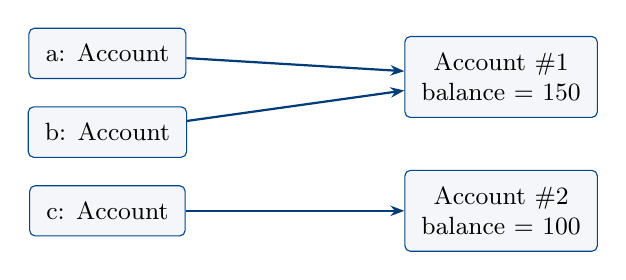
\begin{tikzpicture}
\node[draw=bkblue,rounded corners=2pt,fill=codebg,align=center,inner sep=6pt,font=\small] (a) at (0,0) {a: Account};
\node[draw=bkblue,rounded corners=2pt,fill=codebg,align=center,inner sep=6pt,font=\small] (b) at (0,-1) {b: Account};
\node[draw=bkblue,rounded corners=2pt,fill=codebg,align=center,inner sep=6pt,font=\small] (c) at (0,-2) {c: Account};
\node[draw=bkblue,rounded corners=2pt,fill=codebg,align=center,inner sep=6pt,font=\small] (o1) at (5,-0.3) {Account \#1\\[0pt] balance = 150};
\node[draw=bkblue,rounded corners=2pt,fill=codebg,align=center,inner sep=6pt,font=\small] (o2) at (5,-2) {Account \#2\\[0pt] balance = 100};
\draw[ref] (a) -- (o1);
\draw[ref] (b) -- (o1);
\draw[ref] (c) -- (o2);
\end{tikzpicture}}

\column{0.3\textwidth}
\raggedright
\begin{contextbox}{Output}\begin{lstlisting}[style=code]
150 150 100
true false
\end{lstlisting}
\end{contextbox}
\end{columns}
\vspace{0.8em}
\small a and b share one object. c refers to a separately constructed account with its own balance.
\par\srcline{\href{../../weeks/week-5.html}{Course website: Week 5}. Complete programs accompany this deck.}

\end{frame}

\section{Team round 2: spot the errors}

\begin{frame}[fragile]{Spot the errors 1: Java (5 min)}
\begin{discussionbox}{Contract}\small After depositing 50 into a, balances must be 150 and 200.\end{discussionbox}
\begin{columns}[T,onlytextwidth]
\column{0.48\textwidth}
\raggedright
\begin{lstlisting}[style=bad,language=Java,numbers=left,numberstyle=\tiny\color{codegray},firstnumber=1,numbersep=0.7em]
public class Broken {
    public static void main(String[] args) {
        Account a=new Account(100);
        Account b=new Account(200);
        a.deposit(50);
        System.out.println(a.balance()+" "+b.balance());
    }
\end{lstlisting}

\column{0.48\textwidth}
\raggedright
\begin{lstlisting}[style=bad,language=Java,numbers=left,numberstyle=\tiny\color{codegray},firstnumber=8,numbersep=0.7em]
}
class Account {
    private static int cents;
    Account(int cents) { cents=cents; }
    void deposit(int amount) { cents=amount; }
    int balance() { return cents; }
}
\end{lstlisting}

\end{columns}

\end{frame}

\begin{frame}[fragile]{Spot the errors 1: answers}
\begin{columns}[T,onlytextwidth]
\column{0.58\textwidth}
\raggedright
\begin{contextbox}{The repairs}\footnotesize\begin{itemize}[itemsep=0.45em]\item \textbf{L10:} Use an instance field: different accounts need separate balances.\item \textbf{L11:} Assign the parameter to this.cents.\item \textbf{L12:} Add the deposit rather than replacing the balance.\end{itemize}\end{contextbox}
\column{0.38\textwidth}
\raggedright
\badlabel{Original program}\begin{lstlisting}[style=code]
50 50
\end{lstlisting}
\goodlabel{After the repairs}\begin{lstlisting}[style=code]
150 200
\end{lstlisting}

\end{columns}
\par\srcline{\href{../../weeks/week-5.html}{Course website: Week 5}. Complete programs accompany this deck.}

\end{frame}

\begin{frame}[fragile]{Spot the errors 2: Python (5 min)}
\begin{discussionbox}{Contract}\small The accounts must have independent histories, and print(a) must produce 150.\end{discussionbox}
\begin{columns}[T,onlytextwidth]
\column{0.48\textwidth}
\raggedright
\begin{lstlisting}[style=bad,language=Py,numbers=left,numberstyle=\tiny\color{codegray},firstnumber=1,numbersep=0.7em]
class Account:
    deposits=[]
    def __init__(self, cents): self.cents=cents
    def deposit(self, amount):
        self.deposits.append(amount)
        self.cents=amount
    def __str__(self): print(self.cents)
\end{lstlisting}

\column{0.48\textwidth}
\raggedright
\begin{lstlisting}[style=bad,language=Py,numbers=left,numberstyle=\tiny\color{codegray},firstnumber=8,numbersep=0.7em]

a=Account(100)
b=Account(200)
a.deposit(50)
print(a.cents,b.cents)
print(b.deposits)
print(a)
\end{lstlisting}

\end{columns}

\end{frame}

\begin{frame}[fragile]{Spot the errors 2: answers}
\begin{columns}[T,onlytextwidth]
\column{0.58\textwidth}
\raggedright
\begin{contextbox}{The repairs}\footnotesize\begin{itemize}[itemsep=0.45em]\item \textbf{L2:} Allocate a fresh deposit list inside \_\_init\_\_ for each account.\item \textbf{L6:} Add to the current balance instead of replacing it.\item \textbf{L7:} Return a string from \_\_str\_\_; printing inside it returns None.\end{itemize}\end{contextbox}
\column{0.38\textwidth}
\raggedright
\badlabel{Original program}\begin{lstlisting}[style=code]
50 200
[50]
50
TypeError: __str__ returned non-string (type NoneType)
\end{lstlisting}
\goodlabel{After the repairs}\begin{lstlisting}[style=code]
150 200
[]
150
\end{lstlisting}

\end{columns}
\par\srcline{\href{../../weeks/week-5.html}{Course website: Week 5}. Complete programs accompany this deck.}

\end{frame}

\section{Team round 3: predict the output}

\begin{frame}[fragile]{Predict 1: Aliasing, then replacement}
\begin{columns}[T,onlytextwidth]
\column{0.62\textwidth}
\raggedright
\begin{lstlisting}[style=code,language=Java]
Box a=new Box(2);
Box b=a;
b.side=3;
System.out.println(a.volume());
b=new Box(4);
System.out.println(a.volume()+" "+b.volume());
class Box {
    int side;
    Box(int side) { this.side=side; }
    int volume() { return side*side*side; }
}
\end{lstlisting}

\column{0.34\textwidth}
\raggedright
\begin{discussionbox}{Three minutes}\small Write every line in order. Explain the first state change, alias, dispatch decision or exception that controls the result. Then propose one change that alters the output.\end{discussionbox}
\end{columns}
\par\srcline{\href{../../weeks/week-5.html}{Course website: Week 5}. Complete programs accompany this deck.}

\end{frame}

\begin{frame}[fragile]{Predict 1: answer}
\begin{columns}[T,onlytextwidth]
\column{0.42\textwidth}
\raggedright
\begin{lstlisting}[style=code]
27
27 64
\end{lstlisting}

\column{0.54\textwidth}
\raggedright
\begin{contextbox}{Why}\small The first assignment shares a box. The later constructor creates a new box for b; a still refers to the side-3 box.\end{contextbox}
\end{columns}
\par\srcline{\href{../../weeks/week-5.html}{Course website: Week 5}. Complete programs accompany this deck.}

\end{frame}

\begin{frame}[fragile]{Predict 2: A counter is not an identity}
\begin{columns}[T,onlytextwidth]
\column{0.62\textwidth}
\raggedright
\begin{lstlisting}[style=code,language=Py]
class Ticket:
    issued=0
    def __init__(self):
        Ticket.issued+=1
        self.number=Ticket.issued
a,b=Ticket(),Ticket()
c=a
c.number=9
print(a.number,b.number,Ticket.issued)
print(a is c,a is b)
\end{lstlisting}

\column{0.34\textwidth}
\raggedright
\begin{discussionbox}{Three minutes}\small Write every line in order. Explain the first state change, alias, dispatch decision or exception that controls the result. Then propose one change that alters the output.\end{discussionbox}
\end{columns}
\par\srcline{\href{../../weeks/week-5.html}{Course website: Week 5}. Complete programs accompany this deck.}

\end{frame}

\begin{frame}[fragile]{Predict 2: answer}
\begin{columns}[T,onlytextwidth]
\column{0.42\textwidth}
\raggedright
\begin{lstlisting}[style=code]
9 2 2
True False
\end{lstlisting}

\column{0.54\textwidth}
\raggedright
\begin{contextbox}{Why}\small issued counts constructor calls. c aliases a, so changing c.number changes a.number without creating a third ticket.\end{contextbox}
\end{columns}
\par\srcline{\href{../../weeks/week-5.html}{Course website: Week 5}. Complete programs accompany this deck.}

\end{frame}

\section{Team round 4: write the code}

\begin{frame}[fragile]{Code it: specification}
\begin{discussionbox}{A bank account with a precise contract}\small Read the initial non-negative balance. Then process D amount or W amount until Q. Refuse non-positive amounts and withdrawals above the balance. Print OK or Refused for every command, then Balance: N. Use integer cents.\end{discussionbox}
\begin{columns}[T,onlytextwidth]
\column{0.48\textwidth}
\raggedright
\neutrallabel{Example input}\begin{lstlisting}[style=code]
1000
D 500
W 200
Q
\end{lstlisting}

\column{0.48\textwidth}
\raggedright
\neutrallabel{Expected output}\begin{lstlisting}[style=code]
OK
OK
Balance: 1300
\end{lstlisting}

\end{columns}
\small Eight minutes. One Java team and one Python team at the keyboard. Other teams produce a boundary test and explain which wrong implementation it would expose.
\end{frame}

\begin{frame}[fragile]{Code it: Java solution (1/3)}
\begin{lstlisting}[style=code,language=Java,numbers=left,numberstyle=\tiny\color{codegray},firstnumber=1,numbersep=0.7em]
import java.util.Scanner;
public class Bank {
    public static void main(String[] args) {
        Scanner sc = new Scanner(System.in);
        BankAccount acc = new BankAccount(sc.nextInt());
        String command = sc.next();
        while (!command.equals("Q")) {
            int amount = sc.nextInt();
            boolean ok;
            if (command.equals("D")) {
                ok = acc.deposit(amount);
            } else {
                ok = acc.withdraw(amount);
            }
            System.out.println(ok ? "OK" : "Refused");
\end{lstlisting}
\par\srcline{\href{../../weeks/week-5.html}{Course website: Week 5}. Complete programs accompany this deck.}

\end{frame}

\begin{frame}[fragile]{Code it: Java solution (2/3)}
\begin{lstlisting}[style=code,language=Java,numbers=left,numberstyle=\tiny\color{codegray},firstnumber=16,numbersep=0.7em]
            command = sc.next();
        }
        System.out.println("Balance: " + acc.getBalance());
    }
}
class BankAccount {
    private int balance;
    public BankAccount(int startingBalance) {
        this.balance = startingBalance;
    }
    public boolean deposit(int cents) {
        if (cents <= 0) {
            return false;
        }
        this.balance += cents;
\end{lstlisting}
\par\srcline{\href{../../weeks/week-5.html}{Course website: Week 5}. Complete programs accompany this deck.}

\end{frame}

\begin{frame}[fragile]{Code it: Java solution (3/3)}
\begin{lstlisting}[style=code,language=Java,numbers=left,numberstyle=\tiny\color{codegray},firstnumber=31,numbersep=0.7em]
        return true;
    }
    public boolean withdraw(int cents) {
        if (cents <= 0 || cents > this.balance) {
            return false;
        }
        this.balance -= cents;
        return true;
    }
    public int getBalance() {
        return this.balance;
    }
}
\end{lstlisting}
\par\srcline{\href{../../weeks/week-5.html}{Course website: Week 5}. Complete programs accompany this deck.}

\end{frame}

\begin{frame}[fragile]{Code it: Python solution (1/2)}
\begin{lstlisting}[style=code,language=Py,numbers=left,numberstyle=\tiny\color{codegray},firstnumber=1,numbersep=0.7em]
class BankAccount:
    def __init__(self, starting):
        self.__balance = starting
    def deposit(self, cents):
        if cents <= 0:
            return False
        self.__balance += cents
        return True
    def withdraw(self, cents):
        if cents <= 0 or cents > self.__balance:
            return False
        self.__balance -= cents
        return True
    def balance(self):
        return self.__balance
\end{lstlisting}
\par\srcline{\href{../../weeks/week-5.html}{Course website: Week 5}. Complete programs accompany this deck.}

\end{frame}

\begin{frame}[fragile]{Code it: Python solution (2/2)}
\begin{lstlisting}[style=code,language=Py,numbers=left,numberstyle=\tiny\color{codegray},firstnumber=16,numbersep=0.7em]
acc = BankAccount(int(input()))
line = input()
while line != "Q":
    parts = line.split()
    amount = int(parts[1])
    if parts[0] == "D":
        ok = acc.deposit(amount)
    else:
        ok = acc.withdraw(amount)
    if ok:
        print("OK")
    else:
        print("Refused")
    line = input()
print("Balance: " + str(acc.balance()))
\end{lstlisting}
\par\srcline{\href{../../weeks/week-5.html}{Course website: Week 5}. Complete programs accompany this deck.}

\end{frame}

\begin{frame}{Code it: the tests}
\footnotesize {\scriptsize A slash separates input lines; (blank) denotes an empty line.\par}\medskip \textbf{Test 1}\par \code{1000 / D 500 / W 200 / Q}\par \textbf{Output:} \code{OK / OK / Balance: 1300}\par\medskip \textbf{Test 2}\par \code{100 / W 500 / D -5 / D 50 / Q}\par \textbf{Output:} \code{Refused / Refused / OK / Balance: 150}\par\medskip \textbf{Test 3}\par \code{0 / Q}\par \textbf{Output:} \code{Balance: 0}\par\medskip \textbf{Test 4}\par \code{250 / W 250 / W 1 / D 0 / Q}\par \textbf{Output:} \code{OK / Refused / Refused / Balance: 0}\par\medskip \keyline{Explain why each test is present, not only whether it passes.}
\end{frame}

\section{Wrapping up}

\begin{frame}{What you should now be able to explain}
\begin{itemize}[itemsep=0.6em]\item Distinguish class state from instance state.\item Trace references separately from objects.\item Use constructors, this/self, enums and string representations.\item Explain switch-expression values and the order of guarded cases.\end{itemize}\vfill\small Return to the matching week page for runnable examples and further practice. Bring one unresolved prediction or counterexample to the next class.\par\srcline{\href{../../weeks/week-5.html}{Course website: Week 5}. Complete programs accompany this deck.}

\end{frame}

\end{document}
